\chapter{Discussion and Future Work}
\label{discussion}
\overridetextsize

\section{Addressing Low-Resolution Images}

One possible reason for the inferior detection performance on CIFAR-10 compared
to higher resolution datasets like ImageNet or Dogs vs. Cats, as shown in table
\ref{tab:detection_results}, is the relative size of the adversarial
perturbations required to fool the model. Lower-resolution images, such as those
in CIFAR-10, have fewer pixels and therefore require a more significant
proportion of pixels to be changed to create an adversarial example. This more
significant proportion of pixels changed can make the adversarial perturbations
more noticeable to the human eye. However, it also makes the perturbations more
robust to the random noise added to the image in the proposed method.
Additionally, the lower resolution of CIFAR-10 images may also impact the
ability of the model to classify the image accurately. This is because
lower-resolution images contain less visual information and may have less detail
than higher-resolution images. This lack of detail can make it harder for the
model to identify the important features for classification, which can make the
model more susceptible to adversarial examples. To improve the detection
performance on CIFAR-10, it may be necessary to use a more considerable value of
$\kappa$ to increase the amount of random noise added to the image. However,
increasing $\kappa$ too much can lead to the deterioration of normal images,
increasing false positives. Therefore, it is important to find the right balance
between increasing $\kappa$ to improve the detection of adversarial examples and
not causing too much deterioration of normal images.

\clearpage
\section{Adapting to Adaptive Adversaries}

In the experiments presented, I assumed that the adversaries had full knowledge
of the model's parameters but did not attempt to adapt their methods to bypass
the detection. However, if an adversary were to try and bypass the detection
method, they would face a significant challenge as they would need to produce
examples that keep both scores under unknown thresholds, which is considerably
more complex than simply crafting adversarial examples. Additionally, the
proposed method's random nature makes it difficult for adversaries to adapt
their attack and generate examples that maintain their adversarial effects
across varying unknown noise amounts. This makes it highly challenging for
adversaries to produce adversarial examples that generalize and maintain their
effectiveness under the proposed method's unknown and random parameters.

Furthermore, the proposed method's use of two scores for detection also makes it
difficult for an adversary to bypass the detection. By using two scores, the
proposed method creates a two-fold defense against adversarial examples, making
it more difficult for an adversary to find a way to bypass the detection. Using
two scores also allows for detecting a broader range of adversarial examples,
including those that may have been missed by using a single score.

In conclusion, the proposed method's use of random noise and two scores for
detection makes it difficult for adversaries to adapt their methods to bypass
the detection. The proposed method's randomness, unpredictability, and ability
to be easily combined with other existing defense methods make it a powerful
tool for detecting adversarial examples.

\clearpage
\section{Potential Improvements and Next Steps}

\subsection{Peak Detection Analysis}
During my experiments, I wanted to explore different ways of detecting scores
anomalies. One of the ways I briefly experimented with was to plot the scores
differences at each noise intensity step. For example, given ten $\kappa$, I
computed the first-order difference like so:

\begin{align}
    \label{eq:first-order-diff}
    out_i= \lvert \alpha_{i+1} - \alpha_{i} \rvert,
\end{align}
where $\alpha_i$ represents the score result (either $score_1$ or $score_2$ seen
in \ref{eq:score1} and \ref{eq:score2}) at $\kappa_i$ noise intensity.

\begin{figure}[htp]
    \centering
    \subfloat[]{%
        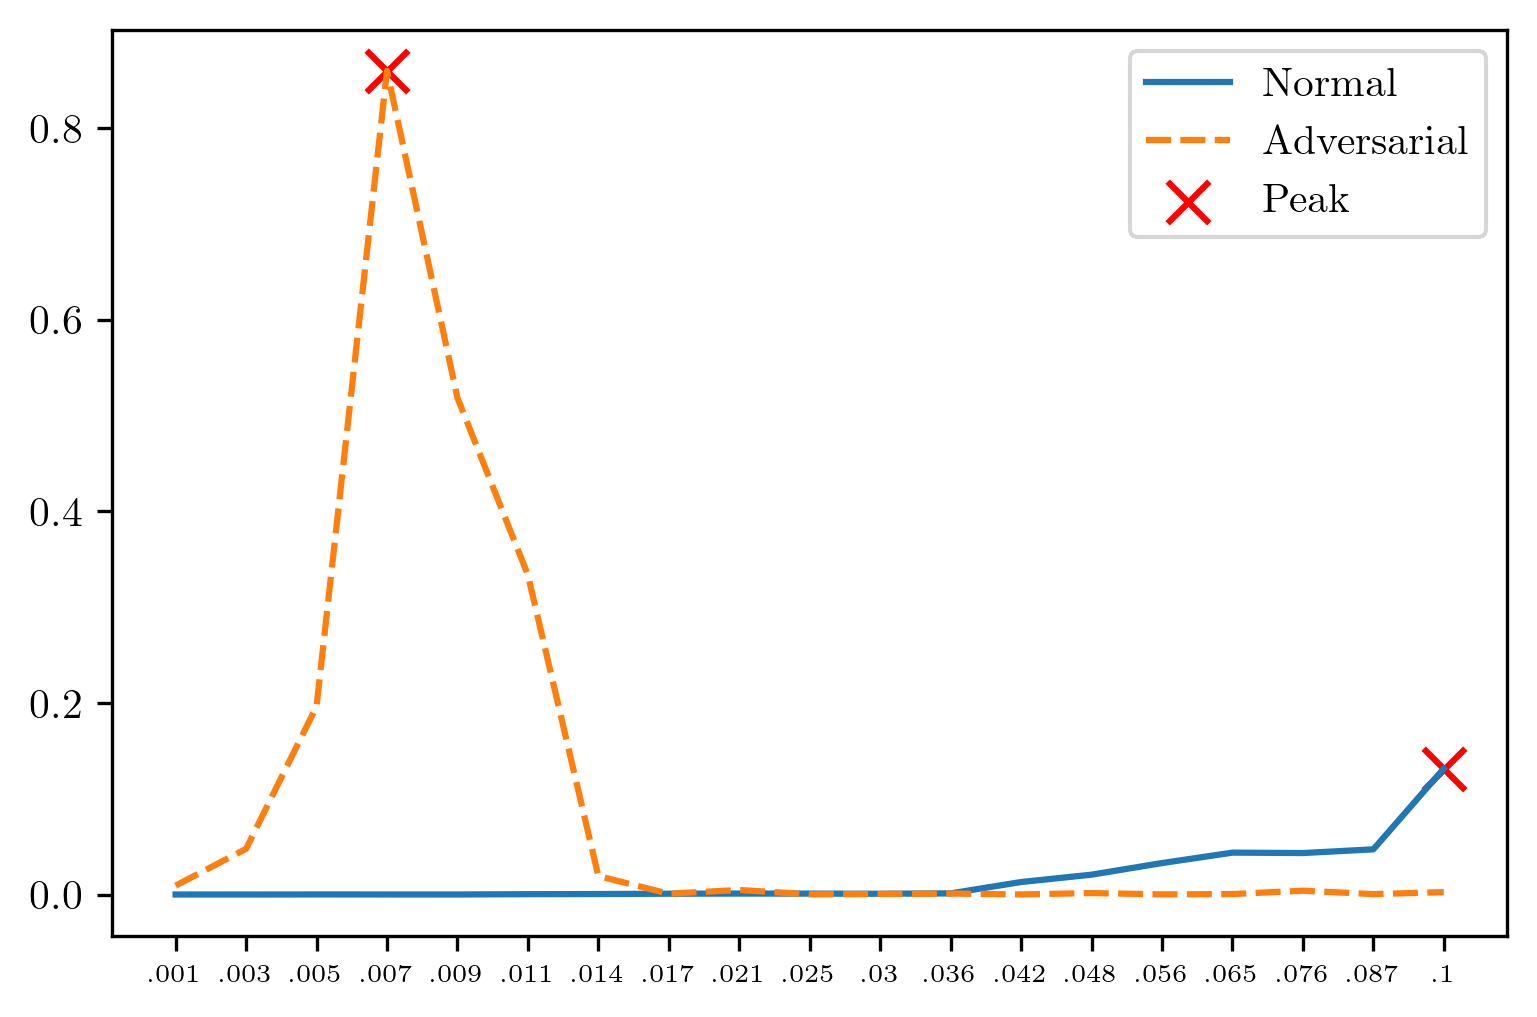
\includegraphics[clip,width=.45\linewidth]{Figures/peaks/1.png}%
    }
    \subfloat[]{%
        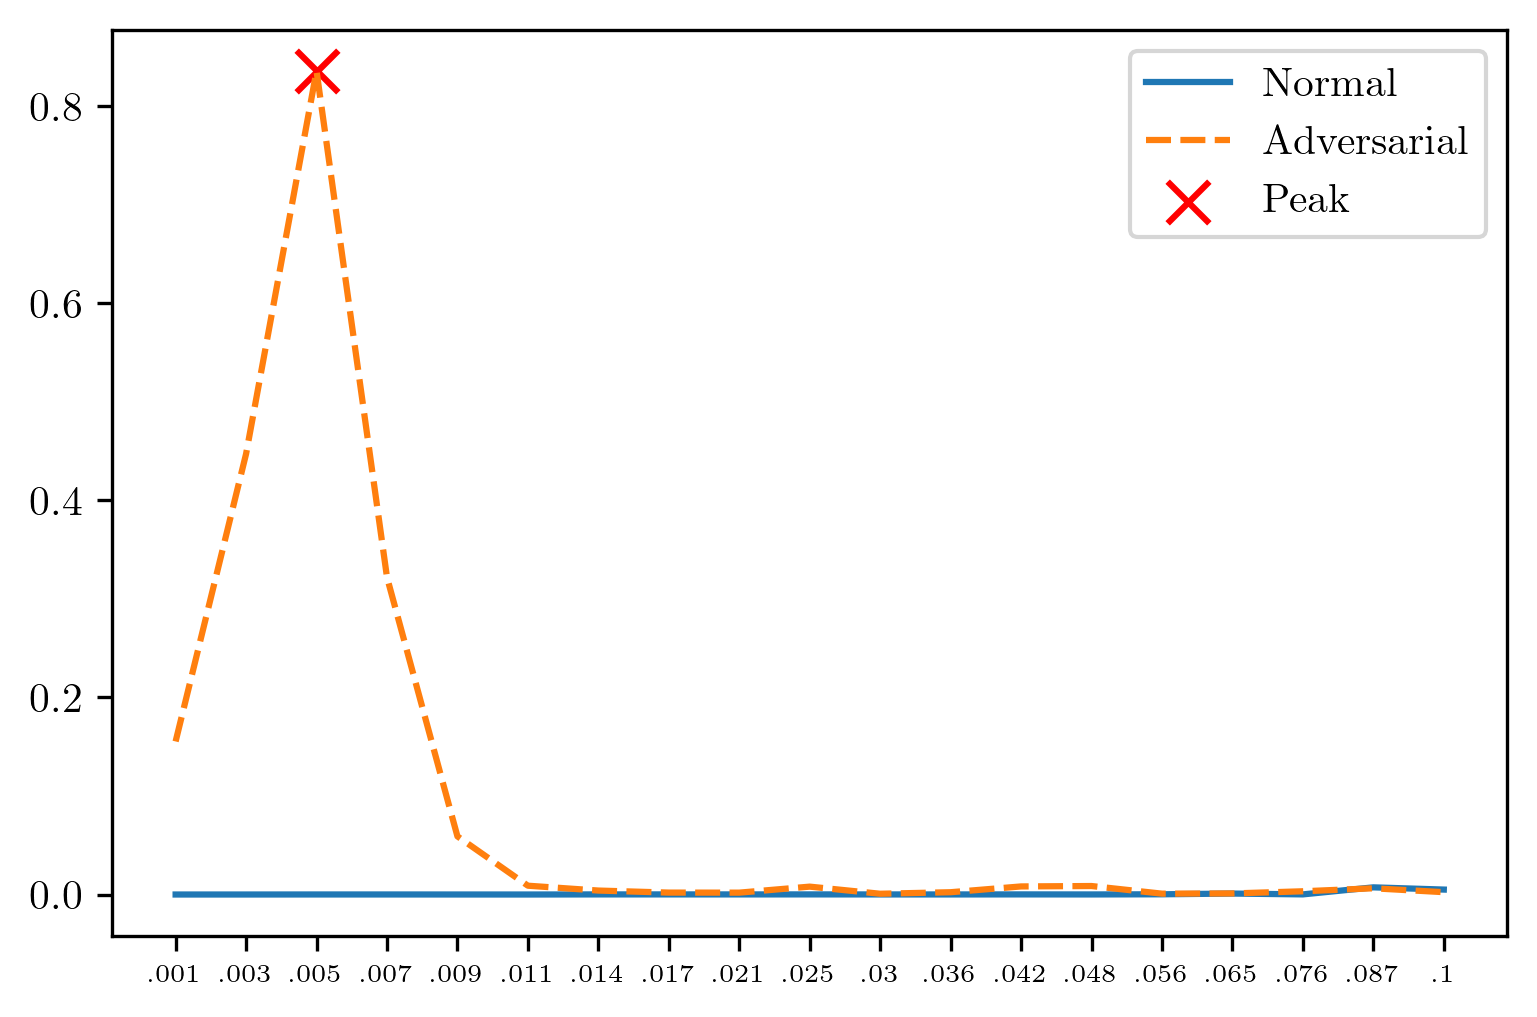
\includegraphics[clip,width=.45\linewidth]{Figures/peaks/3.png}%
    }

    \subfloat[]{%
        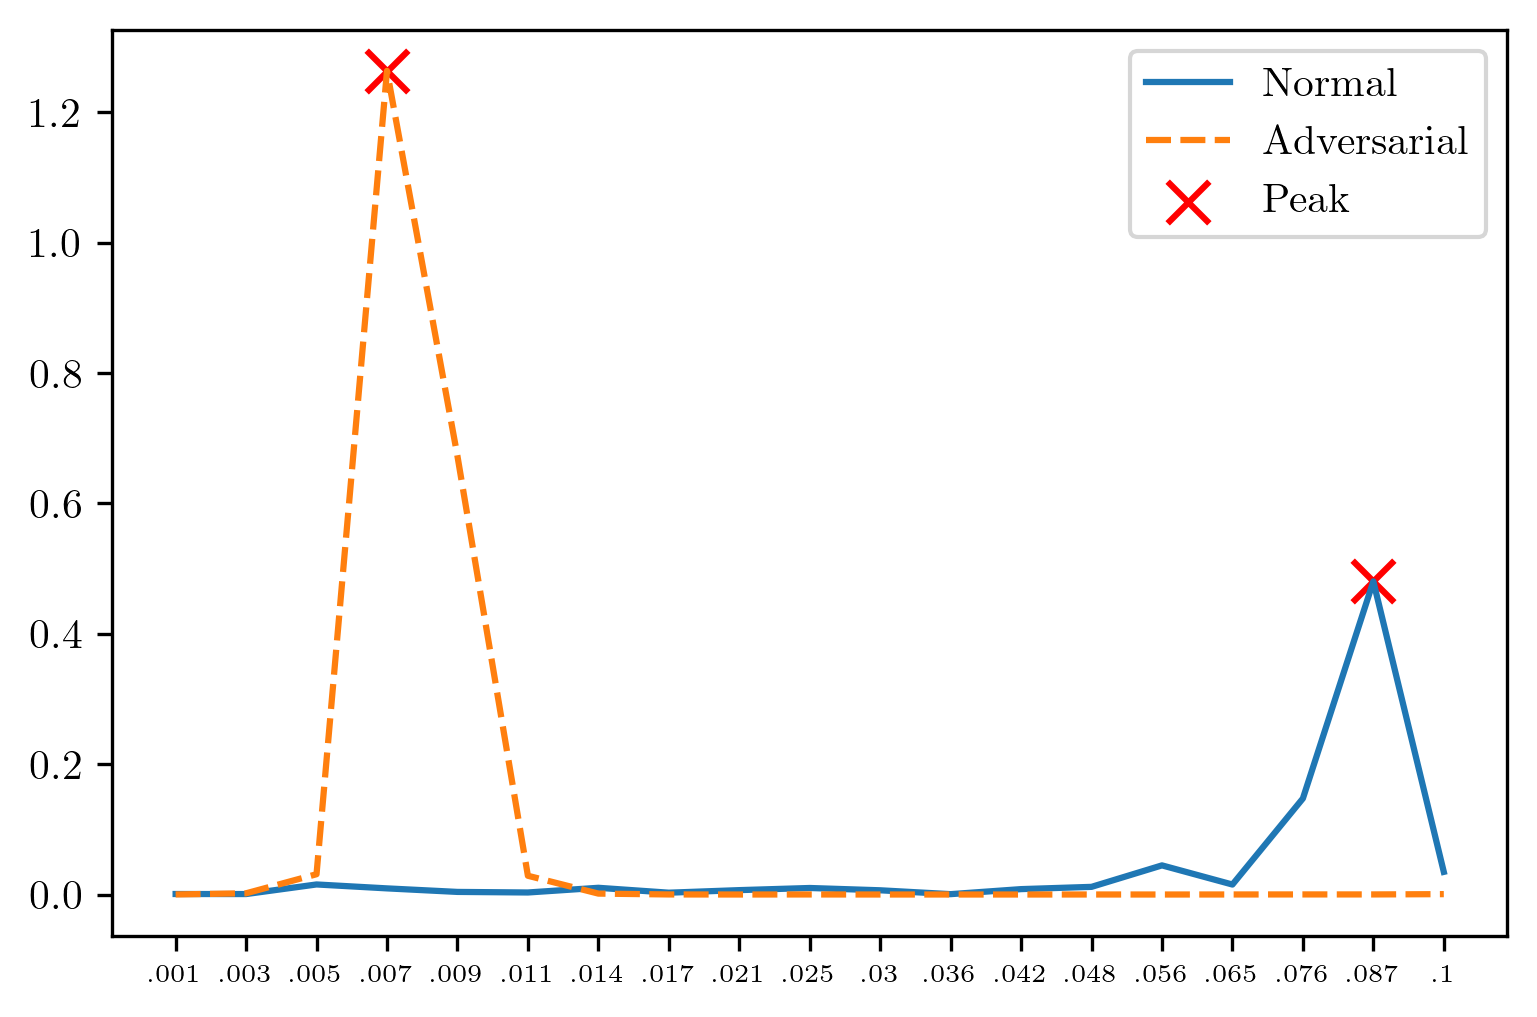
\includegraphics[clip,width=.45\linewidth]{Figures/peaks/13.png}%
    }
    \subfloat[]{%
        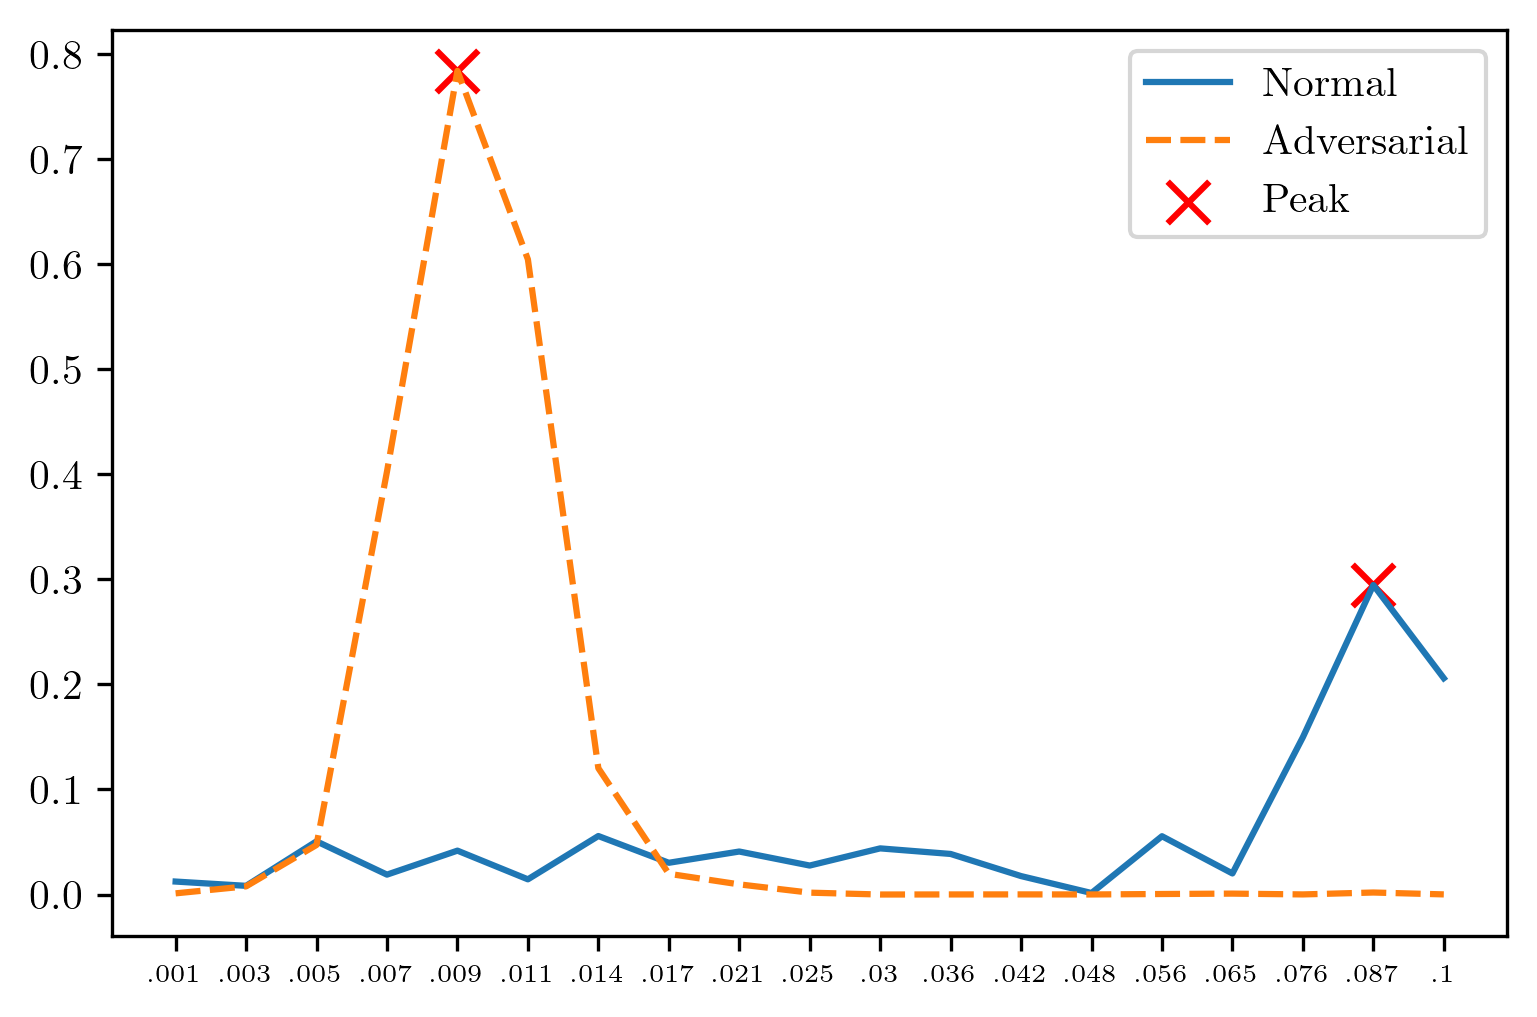
\includegraphics[clip,width=.45\linewidth]{Figures/peaks/20.png}%
    }

    \caption{Peaks observed on normal and adversarial images. Peaks on
        adversarial examples appear to happen at a sooner noise intensity and
        reach a higher value.}
    \label{fig:peaks}
\end{figure}

Figure \ref{fig:peaks} shows the plot of these score differences for four random
images and four adversarial examples generated with different methods. We
observe that the adversarial examples display high peaks earlier than normal
images. In most cases, normal images do not contain peaks at all. This
observation could be used to detect adversarial examples, \emph{e.g.,} by
comparing the intensity of the peaks and when they occur, \emph{i.e.,} when the
first-order difference peaks at an earlier $\kappa$, and at a high magnitude,
this could indicate the adversarial nature of the input.

\subsection{Enhancing Detection Performance with Data Augmentation and Other Techniques}

In this subsection, we explore potential avenues for future research to improve
the detection performance of the proposed method. One promising direction is
incorporating more advanced techniques, such as data augmentation with Gaussian
noise during the training phase. This technique has been shown to be effective
in reducing overfitting and stabilizing models in prior studies, such as the
work done by Zheng et al. \cite{zheng_improving_2016} and Connor et al.
\cite{connor_survey_augmentation_2019}. Furthermore, by incorporating data
augmentation with Gaussian noise, the model's robustness to noise can be further
enhanced, potentially reducing the number of false positives, particularly in
cases where the images are of lower resolution, such as those in the CIFAR-10
dataset. Another interesting area of research is to explore other types of
noise, such as salt and pepper or Poisson noise, and compare the results. This
can help further understand the impact of different types of noise on the
detection performance of the proposed method. Furthermore, it would be
interesting to test the method's robustness against adaptive adversaries capable
of adapting their methods to bypass the detection. This will help to evaluate
the proposed method's ability to detect adversarial examples generated by
adaptive attackers.

Overall, the proposed method provides a promising approach for detecting
adversarial examples, and the results suggest that it has the potential to be
further improved and applied to a wide range of tasks and neural network
architectures.